\vspace{1em}
{\bf IsaViz} is an RDF authoring environment representing RDF models as node-link diagrams. The interpretation of Fresnel in IsaViz is inspired by both Generalized Fisheye Views \cite{furnas06} and Magic Lenses \cite{bier93}. Fresnel lenses, in conjunction with the formats associated with them through groups, are considered as ``genuine'' lenses that modify the visual appearance of objects below them.

Figure \ref{isvFresnelFig} (left) shows the default rendering of a region of an RDF model containing a \rdf{foaf:Person} resource. At this level of magnification, only a few of the many property values associated with the resource are visible. Users need to navigate in the graph in order to get to the values of properties, which can be cumbersome. Alternatively, users can select a Fresnel lens from the list of available lenses loaded in IsaViz through the graphical user interface. The selected lens is then tied to the mouse cursor, and when the lens hovers over a resource that matches its domain, the resource's visual appearance gets modified according to the lens and associated format(s). Resources that match the selected lens' domain are made visually prominent by rendering all other nodes and all arcs using shades of gray with minimum contrast. When the lens hovers over a resource, properties selected by the lens are temporarily rendered with highly-contrasted vivid colors and brought within the current view,
closer to the main resource and reordered clockwise according to the ordering of properties in the lens definition, as illustrated in Figure \ref{isvFresnelFig} (right). Property values revert back to their original state when the lens moves away from the resource. All these visual modifications, including color and position changes, are smoothly animated thanks to the underlying graphical toolkit's animation capabilities \cite{pietriga05}, thus keeping the user's cognitive load low following the principles of perceptual continuity.

\begin{figure}
\begin{tabular}{cc}
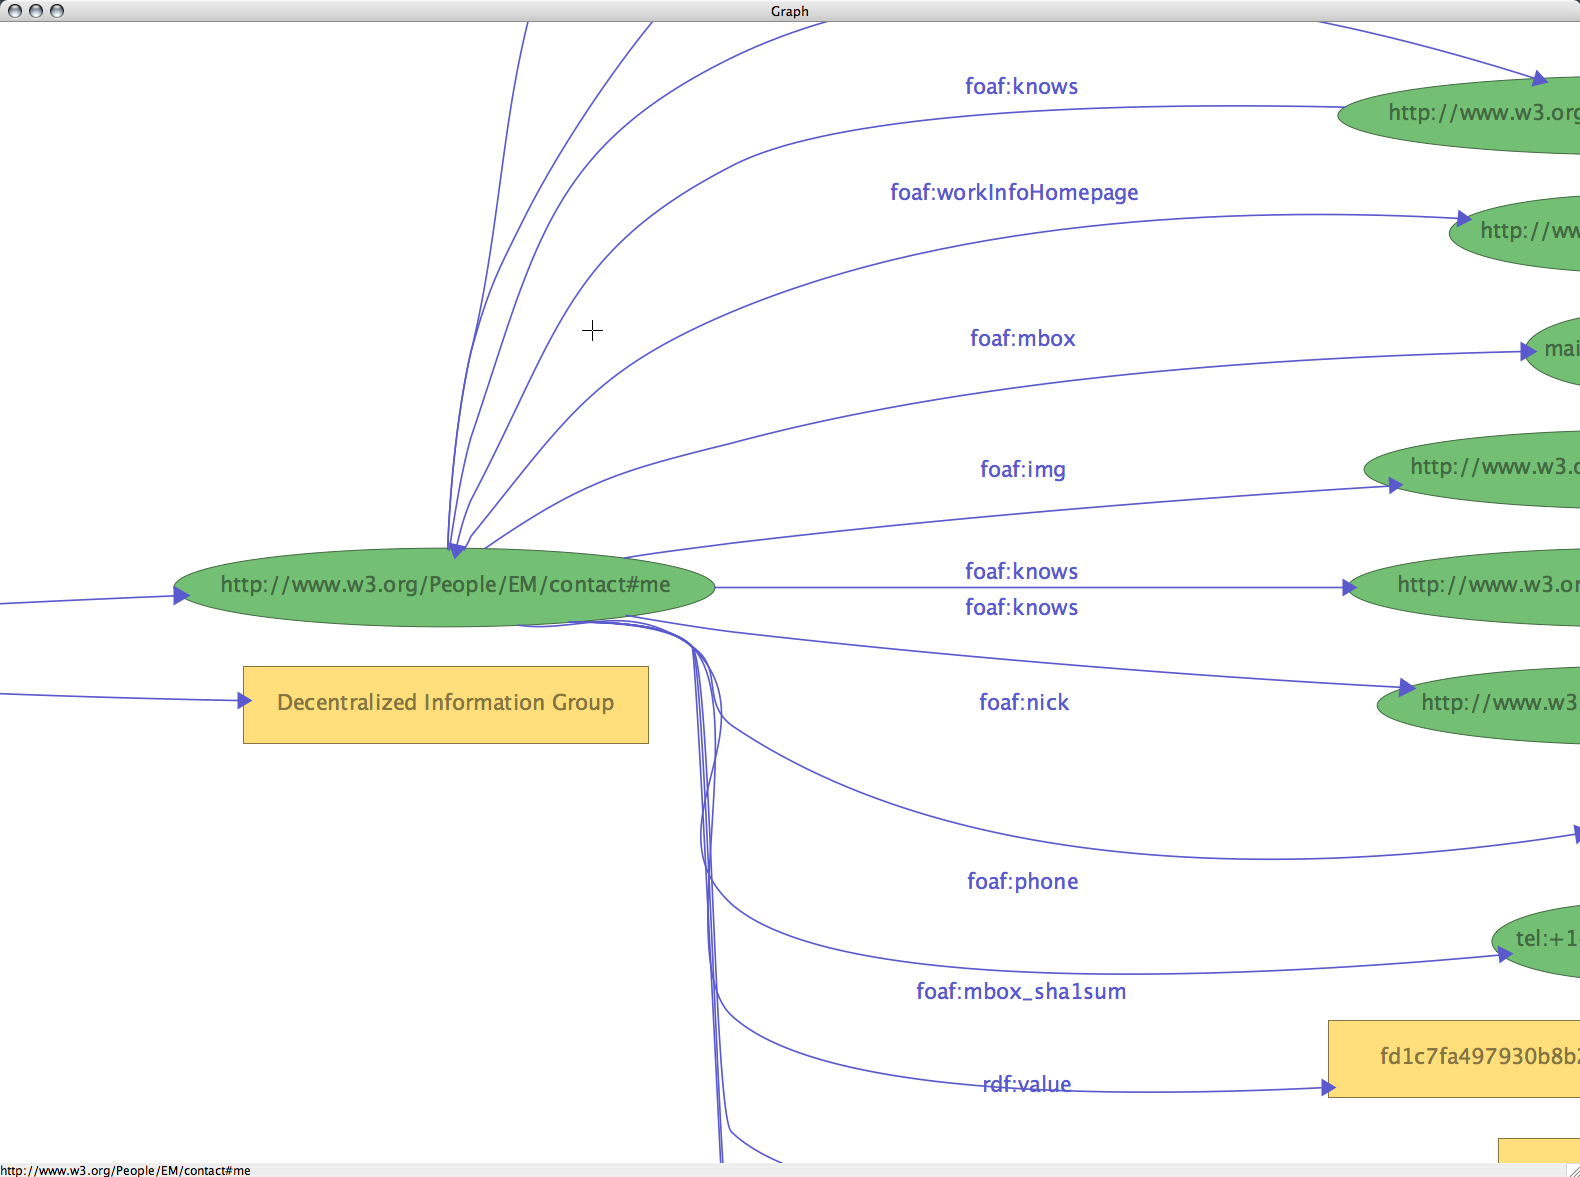
\includegraphics[height=4.45cm]{isavizscreen1.png} \hspace{0.04cm} &
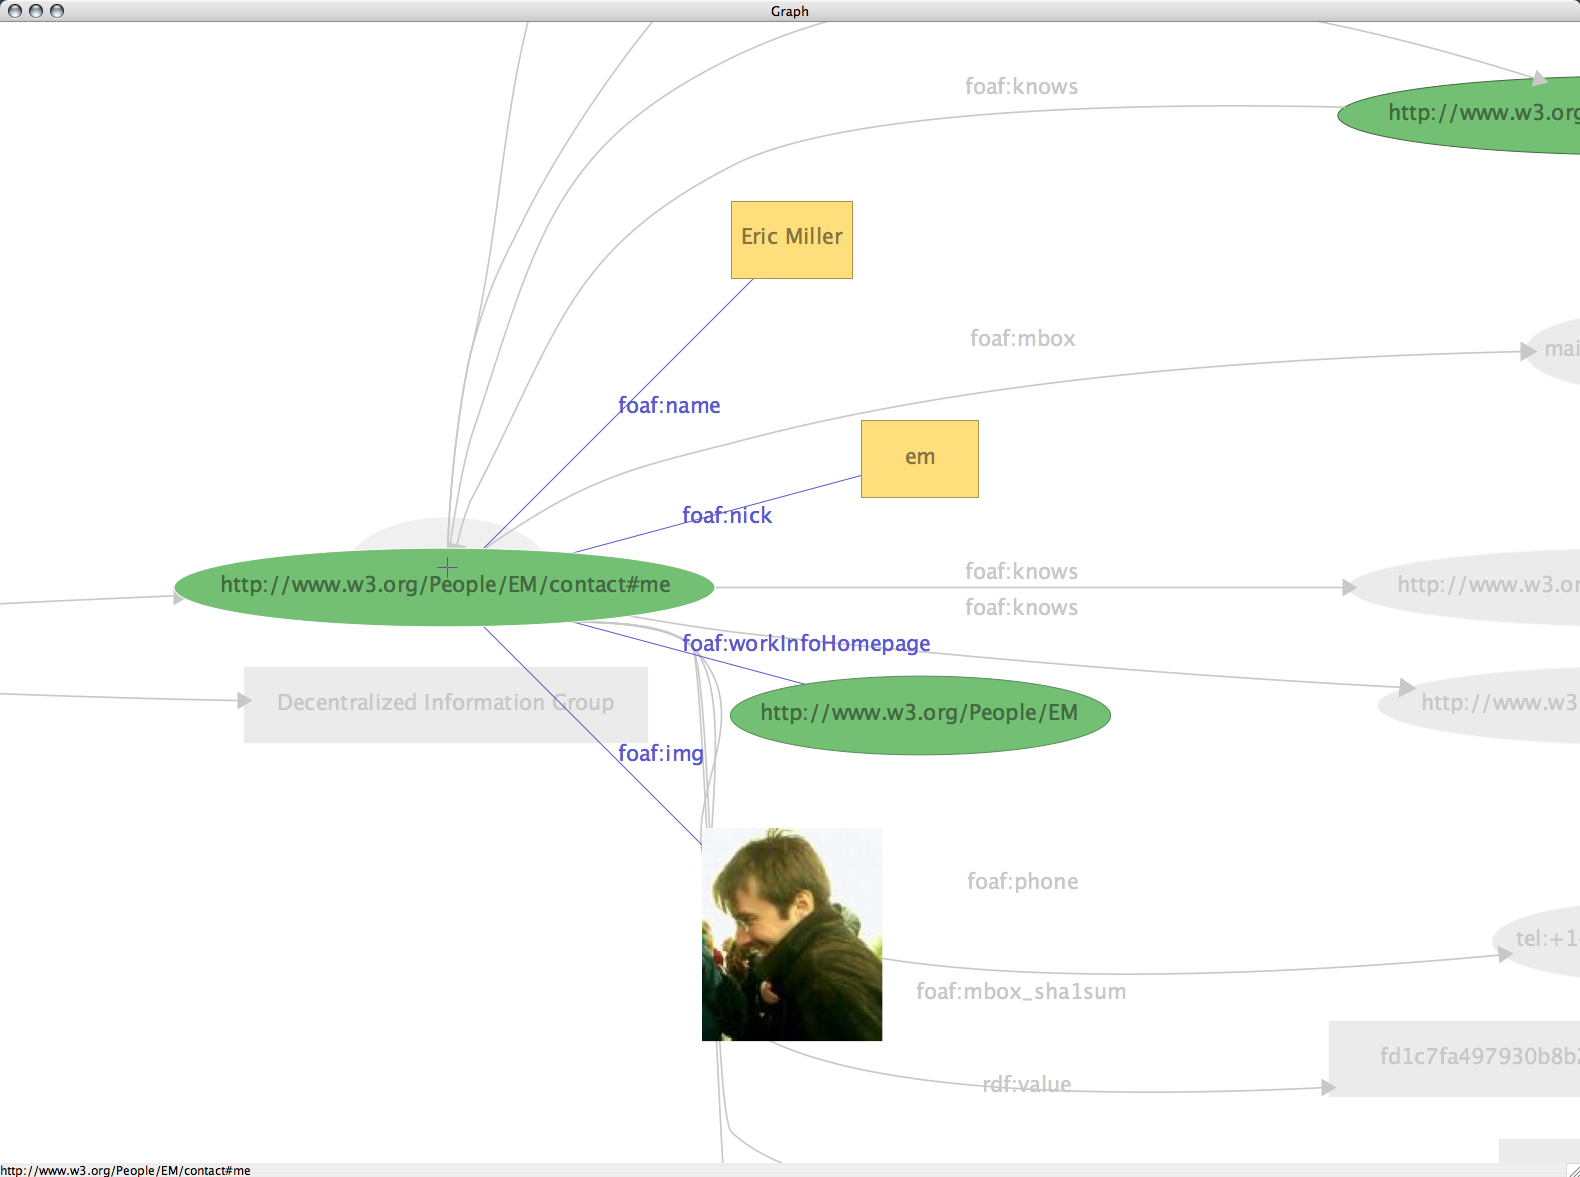
\includegraphics[height=4.45cm]{isavizscreen2.png} \\
\end{tabular}
\vspace{-1em}
\caption{Zoomed-in view of a \rdf{foaf:Person} resource in IsaViz: default presentation (left) and rendered with a Fresnel lens (right)}
\label{isvFresnelFig}
%\vspace{-1em}
\end{figure}

Fresnel core formatting instructions are interpreted as customizations of the original layout and rendering of nodes and links in the diagram. For instance, nodes representing \rdf{foaf:image} property values can be rendered by fetching the actual image from the Web, as illustrated in Figure \ref{isvFresnelFig} (right). The default labels of nodes and arcs can be customized using \rdf{fresnel:label} instructions. In case a resource is the subject of multiple statements involving the same property or properties defined as \rdf{fresnel:mergeProperties}, the arcs and nodes representing these statements can be merged as a single arc and node with all values within that node, optionally separated by text as specified in \rdf{fresnel:contentBefore}, \rdf{fresnel:contentAfter} and related formatting instructions.
